\documentclass[10pt,twoside]{article}

\usepackage{geometry}
 \geometry{
 a4paper,
 total={170mm,257mm},
 left=20mm,
 top=20mm,
 }

%-------------------------------------------------------------------------------  
%Definitions of \mathbb
\newif\ifamsfonts
%if you do not have the AMS font msbm, comment the next line
\amsfontstrue
\ifamsfonts
%definitions of \mathbb with AMS blackboard fonts
\font\tenbbb=msbm10
\font\sevbbb=msbm7
\font\fivbbb=msbm5
\newfam\bbbfam
\textfont\bbbfam=\tenbbb
\scriptfont\bbbfam=\sevbbb
\scriptscriptfont\bbbfam=\fivbbb

\usepackage{microtype}
\usepackage{times}
\usepackage{amssymb,amsmath}
\usepackage{multirow}
\usepackage{graphicx}
\graphicspath{ {images/} }
	\DeclareGraphicsExtensions{.png}
\usepackage{relsize}
\usepackage{amsthm}
\usepackage{scalerel}
\usepackage{enumitem}
\usepackage{color}
\usepackage{soul}
%\usepackage{authblk}

\usepackage[utf8]{inputenc}
\usepackage[spanish,english]{babel}
\selectlanguage{english}

\usepackage{breqn}
\usepackage{subfigure}
\usepackage[toc,page]{appendix}
\usepackage{booktabs}
\usepackage{tabulary}
\newcolumntype{K}[1]%
  {>{\centering\arraybackslash}p{#1}}
\newcolumntype{L}[1]%
  {>{\raggedright\let\newline\\\arraybackslash\hspace{0pt}}m{#1}}
\newcolumntype{C}[1]%
  {>{\centering\let\newline\\\arraybackslash\hspace{0pt}}m{#1}}
\newcolumntype{R}[1]%
 {>{\raggedleft\let\newline\\\arraybackslash\hspace{0pt}}m{#1}}

\usepackage[numbers]{natbib}
\usepackage{mathrsfs}

\usepackage{algorithm}     %http://ctan.org/pkg/algorithms
\usepackage{algpseudocode} %http://ctan.org/pkg/algorithmicx
\setcounter{algorithm}{0}
\renewcommand{\thealgorithm}{\arabic{algorithm}}
\usepackage{caption}
\usepackage{ragged2e}
\usepackage{sidecap} %[outercaption]{sidecap}
\sidecaptionvpos{table}{b}
\usepackage{empheq}

%-------------------------------------------------------------------------------- 
% pdflatex,
% Macros to write hyperlinks
  \ifx\pdfoutput\undefined
        \usepackage[ps2pdf,pagebackref,colorlinks,bookmarksnumbered,
                    breaklinks=true,
                    colorlinks=true,
                    linkcolor=blue,
                    citecolor=red,
                    urlcolor=magenta]{hyperref}
  \hypersetup{
  pdfauthor   = {J.R. Pacha},
  pdftitle    = {TemplateForShortReports},
  pdfsubject  = {Plantilles documents, gener 2010},
  pdfcreator  = {LaTeX2e with hyperref package},
  pdfproducer = {dvips + ps2pdf}
  }
  \else
        \usepackage[pagebackref,colorlinks,bookmarksnumbered,
                    breaklinks=true,
                    colorlinks=true,
                    pdfstartview=FitH,
                    linkcolor=blue,
                    citecolor=red,
                    urlcolor=magenta,
                    pdfstartview={}]{hyperref}
  \hypersetup{
  pdfauthor   = {J.R. Pacha},
  pdftitle    = {TemplateForPapers},
  pdfsubject  = {Plantilles documents, decembre 2010},
  }
  \pdfadjustspacing=1
  \fi
\usepackage{url}

\newcommand{\F}{\ensuremath{\mathbb{F}}}
\newcommand{\R}{\ensuremath{\mathbb{R}}}
\newcommand{\C}{\ensuremath{\mathbb{C}}}
\newcommand{\N}{\ensuremath{\mathbb{N}}}
\newcommand{\Z}{\ensuremath{\mathbb{Z}}}
\newcommand{\h}{\ensuremath{\mathbb{H}}}
\newcommand{\g}{\ensuremath{\mathbb{G}}}
\newcommand{\T}{\ensuremath{\mathbb{T}}}
\newcommand{\Ss}{\ensuremath{\mathbb{S}}}
\newcommand{\uv}{\boldsymbol{u}}
\newcommand{\vv}{\boldsymbol{v}}
\newcommand{\xv}{\boldsymbol{x}}
\let\wt\widetilde

\newcommand{\sgn}{\mathop{\rm sign}\nolimits}
\newtheorem{thm}{Theorem}
\newtheorem{prop}{Proposition}
\newtheorem{cor}{Corollary}
\newtheorem{lemma}{Lemma}
\theoremstyle{remark}
\newtheorem{rem}{Remark}
\newtheorem{example}{Example}
\theoremstyle{definition}
\newtheorem{definition}{Definition}

%%%% Our macros 
\def\cprime{$'$}
\let\wt\widetilde
\newcommand{\diag}{\mathop{\mathrm{diag}}}
\newcommand{\Spp}{\mathop{\mathrm{Sp}}}
\newcommand{\Sp}{\mathop{\mathrm{sp}}}
\newcommand{\spec}{\mathop{\mathrm{Spec}}}
\newcommand{\rmd}{\ensuremath{\mathrm{d}}}
\newcommand{\rme}{\operatorname{e}}
\newcommand{\rmi}{\operatorname{i}}
\renewcommand{\Re}{\mathop{\mathrm{Re}}}
\renewcommand{\Im}{\mathop{\mathrm{Im}}}
\newcommand{\range}{\ensuremath{\mathrm{Range}}}
%\newcommand{\ker}{\ensuremath{\mathrm{Ker}}}
\renewcommand{\baselinestretch}{1.1}

\newcommand{\CH}{\ensuremath{\mathscr{H}}}
\newcommand{\E}{\ensuremath{\mathbb{E}}}
\newcommand{\ES}[1]{\ensuremath{\mathstrut\E_{#1}^{\mathcal{S}}}}
\newcommand{\CS}{\ensuremath{\C^{\mathcal{S}}}}
\newcommand{\hS}{\ensuremath{\h^{\mathcal{S}}}}
\newcommand{\U}{\ensuremath{\mathcal{U}}}
\newcommand{\V}{\ensuremath{\mathcal{V}}}
\newcommand{\Hcal}{\ensuremath{\mathcal{H}}}
\newcommand{\Rcal}{\ensuremath{\mathcal{R}}}
\newcommand{\Tcal}{\ensuremath{\mathcal{T}}}
\newcommand{\wxi}[1]{\ensuremath{\tilde{\xi}_{#1}}}
\newcommand{\wx}[1]{\ensuremath{\tilde{x}_{#1}}}
\newcommand{\wy}[1]{\ensuremath{\tilde{y}_{#1}}}
\newcommand{\wtx}{\ensuremath{\tilde{x}}}
\newcommand{\wty}{\ensuremath{\tilde{y}}}
\newcommand{\wqq}[1]{\ensuremath{\tilde{q}_{#1}}}
\newcommand{\wpp}[1]{\ensuremath{\tilde{p}_{#1}}}
\newcommand{\wtq}{\ensuremath{\tilde{q}}}
\newcommand{\wtp}{\ensuremath{\tilde{p}}}
\newcommand{\arrays}[1]{\renewcommand{\arraystretch}{#1}}

\DeclareMathOperator{\Tr}{Tr}

\allowdisplaybreaks

%-------------------------------------------------------------------------------
\begin{document}
\title{Title of the paper}

\author{
\begin{minipage}[c]{0.3\linewidth}
\centering
First Author$^{1}$\\
\url{first.author@e.mail}
%\href{mailto:first.author@e.mail}{first.author@e.mail}
\end{minipage}
\begin{minipage}[c]{0.4\linewidth}
\centering
  Second Author$^{2}$\\
  \url{second.author@e.mail}
  %\href{mailto:second.author@e.mail}{second.author@e.mail}
\end{minipage}\\ [0,3in]
\begin{minipage}[c]{0.4\linewidth}
\centering
  Third Author$^{3}$\\
  \url{third.author@e.mail}
  %\href{mailto:third.author@e.mail}{third.author@e.mail}
\end{minipage}\\
\begin{minipage}[c]{0.9\linewidth}
\centering
\vspace{\baselineskip}\noindent
$^{1}$Dept.~of the 1st author. Institution of the 1st author.\\
  Address of the 1st author.\\
\vspace{0.75\baselineskip}
$^{2}$Dept.~of the 2nd author. Institution of the 2nd author.\\
  Address of the 2nd author.\\
\vspace{0.75\baselineskip}
$^{3}$Dept.~of the 3rd author. Institution of the 3rd author.\\
  Address of the 3rd author.\\
\vspace{0.75\baselineskip}
\end{minipage}}

\date{\today}
%-------------------------------------------------------------------------------
\maketitle

\begin{abstract}
Enter your abstract here.

%\vspace{\baselineskip}
%\noindent
%\textbf{Note:} final published version available at
%\url{https://doi.org/xx.xxxx/}

\end{abstract}

\textbf{keywords:} keyword1, keyword2,...

\tableofcontents
%-------------------------------------------------------------------------------

\section{First section: introduction}\label{sec:1stSection}
\noindent Here goes the introduction of the prpeprint

\section{Second section}\label{sec:2ndSection}
\noindent Write as many sections as you need and quote as many references as you
need. For example~\cite{GoossensMS94}, \cite{KernighanR88}, and
\cite{Stroustrup97}. 

\subsection{Subsection one}\label{sec:1stSubsectionOf1stSection}
\noindent Write as many subsections as you need.

\subsection{Subsection two}\label{sec:2ndSubsectionOf2ndSection}
\noindent Write as many subsections as you need.

\section{Third section}\label{sec:3rdSection}
\noindent Insert as many figures as you need. For example,
Figure~\ref{fig:lissajousCurve} shows the Lissajous curve
\begin{equation}\label{eq:lissajousCurve}
	x(t) = A\sin(\omega_{1} t + \varphi),\qquad\qquad
	y(t) = B\cos(\omega_{2} t),
\end{equation}
with $A = 2$, $B = 1$, $\omega_{1} = 5$, $\omega_{2} = 3$, and $\delta = \pi/4$.

\begin{figure}[!h]
\centering
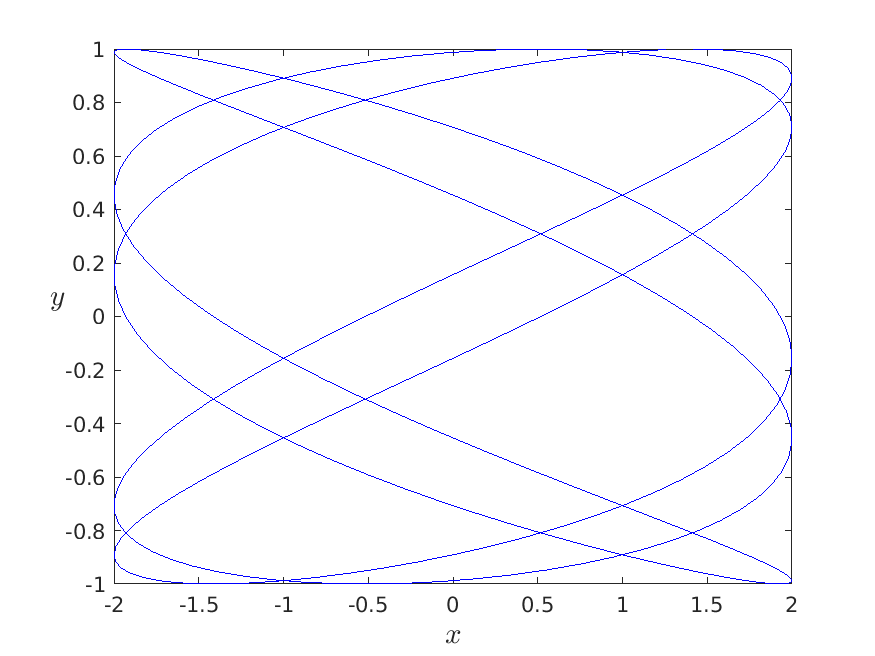
\includegraphics[scale=0.75]{lissajousCurve}
\caption{Plot of Lissajous curve~\eqref{eq:lissajousCurve}.} 
\label{fig:lissajousCurve}
\end{figure}

\section*{Acknowledgments}
\noindent This work was partially supported by\ldots

%\section*{\refname}
\bibliographystyle{plain}
\bibliography{bibEx}

\appendix
\section{First appendix}
\noindent Write as many appendices as you need.

\end{document}

%%% Local Variables:
%%% mode: latex
%%% TeX-master: t
%%% End:
